% !TeX document-id = {6733db24-1e72-4e93-9311-8aa6468b0c5f}
% !TeX TXS-program:compile = txs:///pdflatex/[--shell-escape]
% % !TEX TS-program = xelatex
% !TEX encoding = UTF-8 Unicode

% Spring 2020 - Summer 2020 - Fall 2020
% Tristan Hill, May 07, 2020 - June 12, 2020 - July 08, 2020 - Novemeber 02, 2020
% Module 11 - Probability and Statistics
% Topic 2 - Characterizing a Population of Data

\documentclass[fleqn]{beamer} % for presentation (has nav buttons at bottom)

\usepackage{/home/thill/Documents/lectures/measurements_lectures/measurements_lectures}

\author{ME3023 - Measurements in Mechanical Systems} % original formatting from Mike Renfro, September 21, 2004

\newcommand{\MNUM}{11\hspace{2mm}} % Module number
\newcommand{\TNUM}{2\hspace{2mm}} % Topic number 
\newcommand{\moduletitle}{Probability and Statistics}
\newcommand{\topictitle}{Z Table Examples} 

\newcommand{\sectiontitleI}{Table of Probability Values }
\newcommand{\sectiontitleII}{Example 1}
\newcommand{\sectiontitleIII}{Example 2}
\newcommand{\sectiontitleIV}{Example 3}

% custom box
\newsavebox{\mybox}

\title{Lecture Module - \moduletitle}

\date{Mechanical Engineering\vspc Tennessee Technological University}

\begin{document}
	
	\lstset{language=MATLAB,basicstyle=\ttfamily\small,showstringspaces=false}
	
	\frame{\titlepage \center\begin{framed}\Large \textbf{Topic \TNUM - \topictitle}\end{framed} \vspace{5mm}}\textsl{}

% Section 0: Outline
\frame{
\large \textbf{Topic \TNUM - \topictitle} \vspace{3mm}\\

\begin{itemize}

	\item \sectiontitleI    \vspc % Section I
	\item \sectiontitleII 	\vspc % Section II
	\item \sectiontitleIII 	\vspc %Section III
	\item \sectiontitleIV 	\vspc %Section IV

\end{itemize}

}

\section{\sectiontitleI}	
	% Section I - Frame I
	\begin{frame}[label=sectionI] \small
		\frametitle{\sectiontitleI}    

		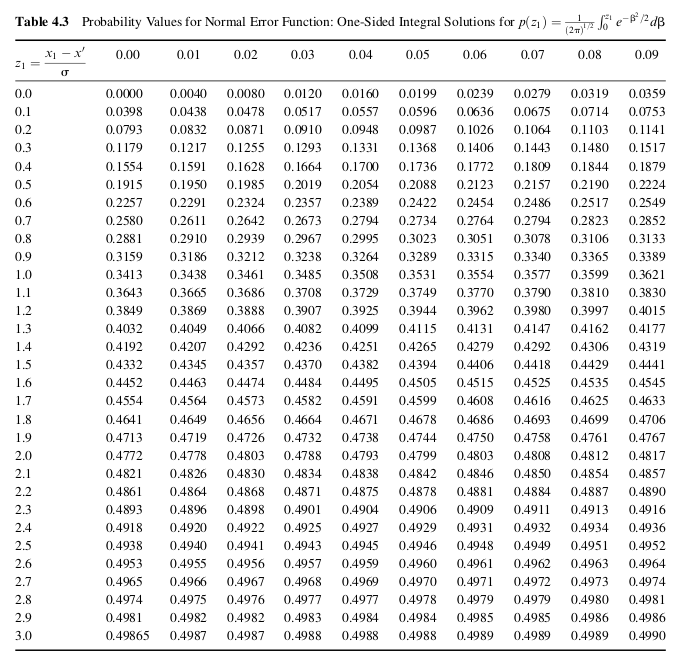
\includegraphics[scale=.3]{topic2_fig2.png}	
		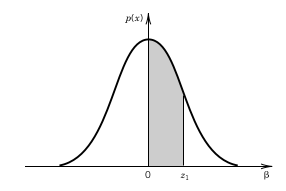
\includegraphics[scale=.3]{topic2_fig3.png}	

	\end{frame}


\section{\sectiontitleII}	
	% Section II - Frame I
	\begin{frame}[label=sectionII] \small
		\frametitle{\sectiontitleII}    
		
		Using the probability values in Table 4.3, show that the probability that a measurement will yield a
value within $x'\pm \sigma$ is $0.6826$ or $68.26\%$.

		\vspace{30mm}
		


	\end{frame}
	




\section{\sectiontitleIII}	

	% Section III - Frame I
	\begin{frame}[label=sectionIII] \small
		\frametitle{\sectiontitleIII}    
		
		Now consider the measurements from the ball bearing factory in topic 1. 
		
		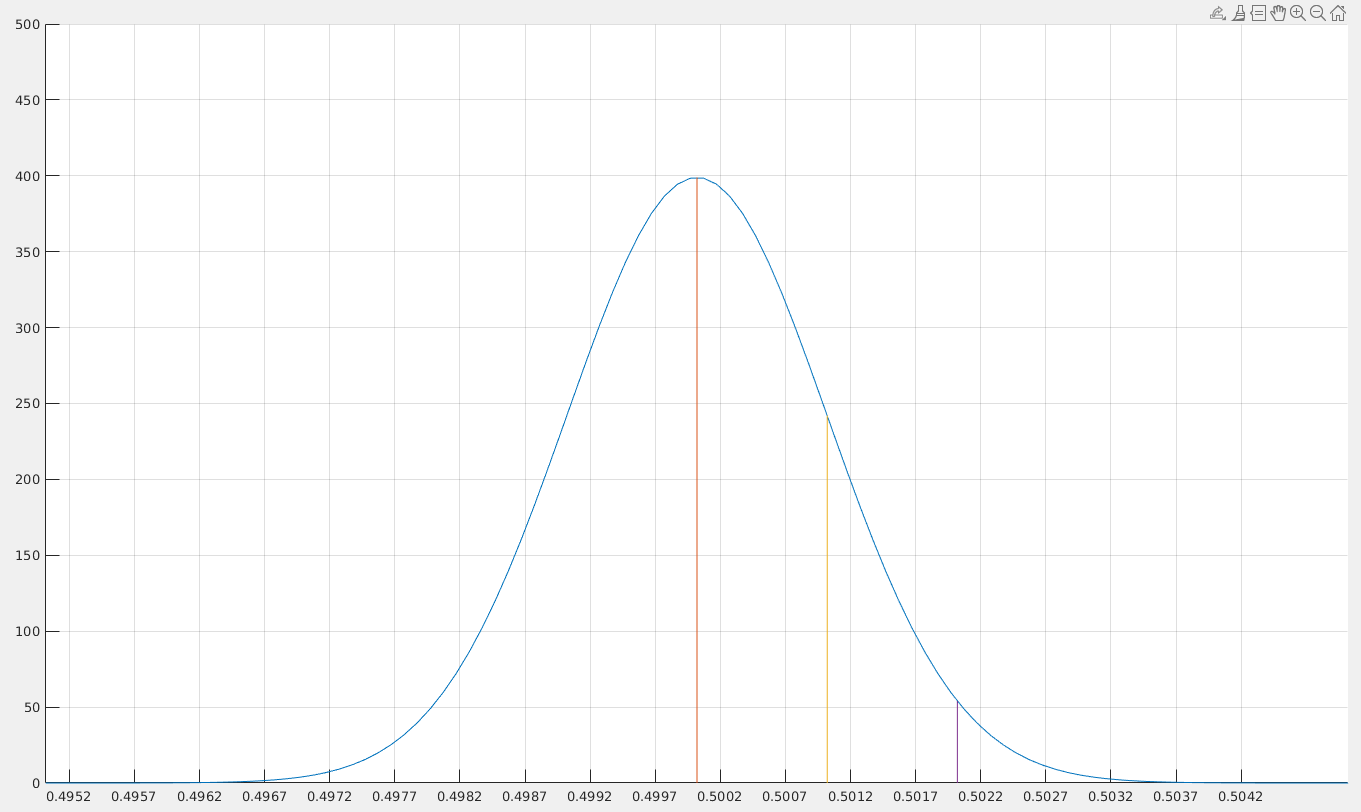
\includegraphics[scale=.2]{topic3_fig1.png}	
	
		
			
		
		\vspace{30mm}
		
		
		

	\end{frame}

% Section III - Frame II
	\begin{frame}[label=sectionIII] \small
		\frametitle{\sectiontitleIII}    
		
		
	If the true mean is 0.5 inches, what is the probability that a individual bearing will measure within 0.45 $\sigma$ of the mean ? What about 0.15 $\sigma$? \\
		\vspace{30mm}

	\end{frame}

% Section III - Frame III
	\begin{frame}[label=sectionIII] \small
		\frametitle{\sectiontitleIII}    
	
		What is the probability that a individual bearing will measure between 0.44 and 0.49 inches? \\\\
			\vspace{30mm}

	\end{frame}

	% Section III - Frame II
	\begin{frame}[label=sectionIII] \small
		\frametitle{\sectiontitleIII}    
		
		If the true mean is 0.5 inches, estimate the uncertainty interval at a probability of 70\%. Also estimate the uncertainty interval at a probability of 90\%.
	What is the probability that a individual bearing will measure within 0.45 $\sigma$ of the mean ? What about 0.15 $\sigma$? \\
		\vspace{30mm}

	\end{frame}
	
	


\section{\sectiontitleIV}	
	% Section IV - Frame I
	\begin{frame}[label=sectionIV] \small
		\frametitle{\sectiontitleIV}    

What is the probability that a individual bearing will measure between 0.40 and 0.44 inches? What is different about this problem? What is the significance of the $z$ value not present in the table?\\\\		
		\vspace{30mm}
	\end{frame}


\end{document}




	





